\chapter{Experiments}
\label{sec:experiments}

% TODO: introduction

\section{Environment and Hardware}
\label{sec:experiments:environmentHardware}
The experiments were conducted on a SLURM cluster using nodes with \num{32} CPU cores, \SI{128}{\giga\byte} RAM and an Nvidia A-100 GPU with \SI{40}{\giga\byte} VRAM. The implementation is written in python 3.10.13. The data was stored in a SQLite database, the database schema can be found in Appendix~\ref{sec:appendix:databaseSchema}.



\section{Experimental Setup}
\label{sec:experiments:setup}

% TODO: introduction?

\subsection{Attribute Sentence Generation}
\label{sec:experiments:setup:sentenceGeneration}
The synthetic dataset that consists of attribute sentences which describe a set of input texts is constructed by prompting an \acs{llm} in a two-step procedure. For this thesis, the open source model Llama 3.2 Instruct\footnote{\url{https://huggingface.co/meta-llama/Llama-3.2-3B-Instruct}}~(\cite{dubeyLlama3Herd2024}) with \num{3} billion parameters has been used. This model has state-of-the-art performance and is freely available, which provides the possibility to run the model directly on the server cluster. Additionally, it improves the reproducibility of the experiments because it is easier to use the exact same model later.
To improve the performance of the sentence generation, the library vLLM\footnote{\url{https://github.com/vllm-project/vllm}} was used to run the model.

The basis for the generation of the attribute sentences are \num{\numAnswersStyleVector} answers from the stack exchange dataset described in Section %~\ref{}. TODO:
For each of the answers, the model is prompted \num{\numPrompts} times to create descriptions of the text with the method presented in Section~\ref{sec:approach:attributeSentenceGeneration}.

For each of the resulting \num{\numStyleDescriptions}, the model is prompted again to convert the description into a list of sentences of the form \enquote{The author is \ldots} or \enquote{The author uses \ldots}. The output of the \ac{llm} is split into sentences using the Natural Language Toolkit\footnote{\url{https://www.nltk.org/}} library (\cite{birdNaturalLanguageProcessing2009}). The naive approach of splitting the sentences at the punctuation would not work because they could contain punctuation with expressions like \enquote{e.g.}.

The model is instructed to avoid negations and examples because they can lead to the sentences having too dissimilar a shape while conveying the same meaning. In addition to this constraint that is stated in the prompt, the final sentences are checked to not include the word \enquote{not}. If they do, they are skipped and not used for further computation. During the experiments, \num{\numSentencesWithNegations} sentences have been filtered for this reason.

After the previous steps, \numStyleSentencesNotUniqueText{} attribute sentences have been produced. After taking into account only unique sentences, \numStyleSentencesText{} attribute sentences are left. Of these, \num{\numStyleSentencesStyle} sentences are style sentences, which means they have been produced by a style prompt, and \num{\numStyleSentencesKnowledge} are knowledge prompts.
% TODO: are style sentences + knowledge sentences = all sentences? if not, explain

\subsection{Clustering}
\label{sec:experiments:setup:clustering}
Although checking for exact duplicates reduces the number of sentences significantly, there are still many sentences that have basically the same meaning, but are not exactly the same. This can lead to the problem that it would not be clear if an attribute sentence has rarely been used to describe the input texts or if the \ac{llm} has just a high syntactic variance in describing one concept.

The solution to this problem that this thesis proposes is to cluster the sentences and use the clusters as attributes by using the sentence that is closest to the center as the representation for the cluster.
The first step for this procedure is to create an embedding of all sentences so they can be compared semantically. The SBERT model \textit{all-MiniLM-L12-v2}\footnote{\url{https://huggingface.co/sentence-transformers/all-MiniLM-L12-v2}} (\cite{reimersSentenceBERTSentenceEmbeddings2019}) was used to create the embeddings.

For the following steps, the style and knowledge sentences have been processed separately to ensure the resulting clusters are either style or knowledge clusters.
The clustering algorithm first computes a radius neighbor graph of all sentences. All sentences that have a cosine similarity higher than \num{\minCosineSimilarity} are considered to be in the same cluster. Subsequently, the clusters are sorted by size and inspected from largest to smallest. If a sentence is included in one cluster, it is removed from all smaller ones. It is important to note that there is no minimum size for a cluster; if a sentence has no neighbors or every one of them is already part of a larger cluster, then the cluster size is one.

% TODO: why 0.85 min similarity?

At this point, there are \num{\numClusters} clusters, \num{\numClustersStyle} of which are style clusters and \num{\numClustersKnowledge} are knowledge clusters. The size of the complete synthetic dataset can be found in Table~\ref{table:syntheticDataset}.

\begin{table}[ht]
  \begin{center}
    \begin{tabular}{lS[table-format=7.0]}
      \toprule
                   & {Number of data points} \\ \midrule
      Answers      & \numAnswersStyleVector  \\
      Prompts      & \numPrompts             \\
      Descriptions & \numStyleDescriptions   \\
      Sentences    & \numStyleSentences      \\
      Clusters     & \numClusters            \\ \bottomrule
    \end{tabular}
  \end{center}
  \caption{The size of the synthetic dataset created for this thesis. The answers are the group-specific input texts that are taken from the Stack Exchange dataset (see Section~\ref{sec:datasets:stackex}). For each answer and prompt, the \ac{llm} is prompted to create the style and knowledge descriptions. The descriptions are converted to attribute sentences by prompting the model again. Finally, the sentences are clustered together by the cosine similarity of their embeddings. The embeddings were produced with an SBERT model (\cite{reimersSentenceBERTSentenceEmbeddings2019}).}
  \label{table:syntheticDataset}
\end{table}

\subsection{Selecting the Attribute Vector Dimensions}
\label{sec:experiments:setup:selection}
The synthetic dataset resulting from the previous steps consists of \num{\numClusters} clusters, which are the potential dimensions of the interpretable attribute vector. This vector however consists of \num{\styleVectorSize} dimensions as established by \citet{patelLearningInterpretableStyle2023}. Therefore, the best clusters have to be selected to be part of the attribute vector. This selection is carried out in multiple steps, which are described in the following section and additionally shown in Figure~\ref{fig:clustering}.

\begin{figure}[h!t]
  \begin{center}
    % \begin{tikzpicture}[
    % arrow tip
    >=Stealth,
    % box style
    box/.style={
        draw,
        rectangle,
        minimum width=50mm,
        minimum height=10mm,
        align=center
      },
    % dashed region style
    dashedbox/.style={
        draw,
        dashed,
        inner sep=6mm
      },
    % default distance between nodes
    node distance=8mm and 12mm
  ]

  % Top layer
  \node[box] (attrib) {Attribute Sentences};
  \node[box, below left=of attrib]  (stySent) {Style Sentences};
  \node[box, below right=of attrib] (knSent)  {Knowledge Sentences};

  % Clustering step
  \node[box, below=of $(stySent)!0.5!(knSent)$] (cluster)
  {Clustering by Cosine Similarity};

  % Resulting clusters
  \node[box, below left=of cluster]  (styCl) {Style Clusters};
  \node[box, below right=of cluster] (knCl)  {Knowledge Clusters};

  % Three sequential steps
  \node[box, below=of $(styCl)!0.5!(knCl)$] (step1)
  {used in maximum number of groups\\minimum usages};
  \node[box, below=of step1] (step2)
  {clusters with a minimum distance to each other};
  \node[box, below=of step2] (step3)
  {clusters with largest difference in agreement levels};

  % Dashed box around those three steps
  \node[dashedbox, fit=(step1)(step2)(step3)] {};

  % Final attribute-vector block
  \node[box, below=of step3] (attrVec) {
    \begin{tabular}{ccc}
      Targeted Style Attributes & Knowledge Attributes & Style Attributes
    \end{tabular}
    \\[2pt]
    \textbf{Attribute Vector}
  };

  % Arrows
  \draw[->] (attrib)  -- (stySent);
  \draw[->] (attrib)  -- (knSent);
  \draw[->] (stySent) -- (cluster);
  \draw[->] (knSent) -- (cluster);
  \draw[->] (cluster) -- (styCl);
  \draw[->] (cluster) -- (knCl);
  \draw[->] (styCl)    -- (step1);
  \draw[->] (knCl)     -- (step1);
  \draw[->] (step1)    -- (step2);
  \draw[->] (step2)    -- (step3);
  \draw[->] (step3)    -- (attrVec);
  \draw[->] (attrVec.west) .. controls +(-15mm,0) and +(-15mm,24mm) .. (stySent.west);

\end{tikzpicture}

    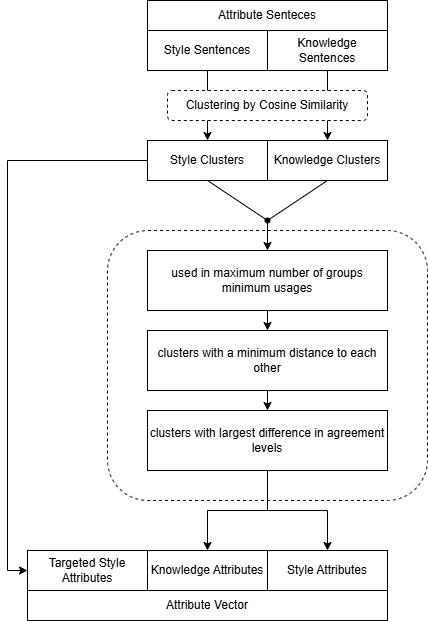
\includegraphics[width=9cm]{figures/clustering_diagram.png}
  \end{center}
  \caption{The approach so far (see Figure~\ref{fig:attributeSentenceGeneration}) has produced about \numStyleSentencesText{} unique attribute sentences. While these sentences are syntactically distinct from each other, semantically they can be very close. To improve the performance of the method proposed in this thesis, similar sentences are clustered. First, all sentences are embedded. Then, sentences with a cosine similarity higher than \num{\minCosineSimilarity} are clustered together while ensuring that every sentence is in exactly one cluster. The clustering is performed separately for style and knowledge sentences. From the resulting \num{\numClustersStyle} style clusters and \num{\numClustersKnowledge} knowledge clusters, the best ones are selected in multiple steps until the final interpretable attribute vector with \num{\styleVectorSize} dimensions is created, where each dimension corresponds to one cluster. The first \num{\numTargetPrompts} dimensions of the attribute vector are selected separately and correspond to the targeted prompts presented in Section~\ref{sec:approach:attributeSentenceGeneration}.}
  \label{fig:clustering}
\end{figure}

\subsubsection{Selection of target attributes}
\label{sec:experiments:setup:selection:targetAttributes}
Following the work of \citet{patelLearningInterpretableStyle2023}, the first \num{\numTargetPrompts} dimensions of the attribute vector will be selected to correspond to the \num{\numTargetPrompts} target prompts, which were described in Section~\ref{sec:approach:attributeSentenceGeneration}.
This is done to ensure that the attribute vector has a robust foundation on some features that are manually selected for being relevant for stylistic research. The ability to automatically create most of the attribute vector is not significantly reduced since the target attributes only account for around \SI{10}{\percent} of its size.

These attributes are found by creating sentences of the form \enquote{The author uses <target>} and embedding them using the same embedding model that has been used to embed the attribute sentences, the all-MiniLM-L12-v2 model.
Afterward, for each sentence, the style cluster with the highest cosine similarity is found. This cluster is then one of the target attributes of the vector.

% TODO: write better?
The knowledge clusters are not taken into account during this selection. Since all style sentences that are produced by the targeted prompts can not be part of any knowledge cluster, any knowledge cluster that has a very high cosine similarity would be an unwanted cluster that should not be chosen at this point.

% TODO: compare to what patel et al. have done?

\subsubsection{Filtering out attributes that occur too frequently}
\label{sec:experiments:setup:selection:filteringOccurance}
An important characteristic of all attributes that are part of the attribute vector is that they are as meaningful as possible and help to distinguish between different groups. To ensure this requirement is met, attributes that describe texts of a too large portion of groups are removed. Based upon the work of \citet{patelLearningInterpretableStyle2023}, the maximum number of groups that can be described by an attribute cluster is \SI{60}{\percent}.

At the same time, the number of clusters that are taken into account for the next selection steps has to be reduced because these steps have a quadratic memory requirement. To quickly reduce the number of clusters, the number of times the cluster was used to describe answers is taken into account. The required number of times used is increased until the resulting number of clusters is small enough. This way, the largest clusters that are not used to describe too many groups are used for the next steps.

To determine how many times a cluster was used to describe an answer, each sentence is only counted once per answer. Multiple prompts could produce the same attribute sentence to describe an answer; counting all of them would however distort the number of usages of the clusters.

\subsubsection{Removing too similar Attributes}
\label{sec:experiments:setup:selection:removeSimilar}
To ensure that the attribute vector covers a wide range of attributes, it is important that the attributes do not cover too similar topics. This is achieved by ensuring that the clusters have a maximum cosine similarity of \num{\maxCosineSimilarity} to each other. This process works by ordering the clusters by occurrence, selecting them one after the other, and deleting all clusters that are too close to the ones that have already been selected.
The cosine similarity is computed between the embeddings of the attribute sentence that is closest to the center of the embedding.

% TODO: explanation why 0.7
\begin{itemize}
  \item patel et al have a maximum cosine similarity of 0.8, I have 0.7
  \item in this case, sentences that have a similarity higher than 0.85 are in the same cluster
  \item a lower maximum similarity guarantees a broader attribute vector
  \item when lower than 0.7, there are not enough attribute candidates
\end{itemize}

\subsubsection{Final Selection} % TODO: better name?
\label{sec:experiments:setup:selection:finalSelection}
The first \num{\numTargetPrompts} dimensions of the attribute vector are the target attributes that were selected in Section~\ref{sec:experiments:setup:selection:targetAttributes}. The next \num{\minNumKnowledgePrompts} dimensions are knowledge clusters, that is, clusters of sentences that were produced by knowledge prompts. The rest of the dimensions are selected in this step to be the ones with the highest difference in agreement levels.

A difference in agreement levels means that the range between responses that fit the attribute well and those that do not is as wide as possible. This further increases the likelihood that the attributes are good at distinguishing between different responses and groups.

% TODO: complete code
% \lstinputlisting[language=Python, caption={Pseudo code for the final cluster selection step.}]{content/05-experiments/final-cluster-selection.py}

First, the similarity between all clusters that remain after the first selection steps is computed. Afterward, for each cluster and each answer, the average similarity to all other clusters that have been used to describe that answer is computed. The result is a rough estimation of the actual similarity between the current attribute sentence and the answer.

Subsequently, the range between the similarity of the most and least similar answers is computed, and the clusters with the highest difference are selected. With the process, the probability of attributes holding meaningful information to distinguish between different groups is increased.

\subsection{\acf{sfam}}
\label{sec:experiments:setup:sfam}
For the creation of the attribute vector, this thesis utilizes the \acl{sfam} proposed by \citet{patelLearningInterpretableStyle2023}. There are however two significant changes in comparison to the original model. For one, DeBERTa-V3-base\footnote{\url{https://huggingface.co/microsoft/deberta-v3-base}} (\cite{he2021deberta}) was used as the base model instead of t5-base. Furthermore, the final output is produced with a regression head with a single output instead of a binary classification head.
% TODO: explain why not deberta-large?
% TODO: what hyperparameters were used?

The final layer of the model proposed by \citet{patelLearningInterpretableStyle2023} has to output neurons; one for positive prediction and one for negative prediction. To get the agreement score, a softmax over the two values is used. In contrast to that, the method presented by this thesis uses a final layer with just one output neuron which has a sigmoid activation function. Therefore, the output of the model is the agreement score without any additional computation step.

The input to the model is truncated to 512 tokens following the work of \citet{patelLearningInterpretableStyle2023}.

\acs{sfam} is trained on the synthetic dataset that was described in the previous sections. The training data is balanced and consists of attribute sentences with one answer from the Stack Exchange Dataset (see Section~\ref{sec:datasets:stackex}), which fits the attribute sentence as a positive sample and one answer which does not fit the sentence as a negative sample. The input to the model is a string of the form \enquote{\(\{\{a\}\}~|||~\{\{t\}\}\)}, where \(a\) is the attribute sentence and \(t\) is the text that is the positive or negative sample.

The selection of the attribute sentences and answers used for training is similar to the process described in Section~\ref{sec:experiments:setup:selection:finalSelection} and differs from \citet{patelLearningInterpretableStyle2023}. They select sentences for training at random and choose a text that is described with the sentence in the synthetic dataset as a positive sample. A negative sample is selected by sampling a text that is described by the sentence with the largest cosine distance to the current sentence.
The potential problem with this process is that the annotation in the synthetic dataset is not perfect and it is possible that the text that are selected as a positive sample do not actually correspond to the sentence.

The method proposed in this thesis instead orders all answers by a heuristic similarity to the sentence and selects one of the most similar to a positive sample and one of the most dissimilar as a negative sample. For each sentence, first the heuristic similarity to each text is computed. This is done by computing the similarity to all attribute vector dimensions that are used to describe the text in the synthetic dataset. The average of these similarities serves as an approximation for the actual similarity.

Subsequently, the answers are ordered by their heuristic similarity to the attribute sentence. The positive training sample is the most similar text where the sentence was used to describe it in the synthetic dataset. The negative training sample is the most dissimilar sentence that was not described by the sentence. If a candidate for the positive sample is not in the top \sfamDataTopPercentText{}, the sentence is not used for the \ac{sfam} training dataset. % TODO: reason
Since the synthetic dataset consists of \numStyleSentencesText{} attribute sentences and the \ac{sfam} training dataset consists of only \num{\sfamTrainingDataSize} samples, it is no problem to discard sentences where the positive sample does not have a sufficiently high heuristic similarity.

The validation and test datasets are produced with the same method. However, while \citet{patelLearningInterpretableStyle2023} sample distinct sets of sentences for the training, validation, and test datasets, for this thesis the input texts themselves are assigned to the different dataset categories. The attribute sentences produced from these texts are also largely distinct, also this is not enforced and simply a side effect of the \ac{llm} using different formulations for the same concepts (see Figure~\ref{fig:sfamDatasetSplit}).
Because of this, \ac{sfam} is tested not only on unseen attribute sentences but on unseen texts as well.

\begin{figure}[ht]
  \begin{center}
    %% Creator: Matplotlib, PGF backend
%%
%% To include the figure in your LaTeX document, write
%%   \input{<filename>.pgf}
%%
%% Make sure the required packages are loaded in your preamble
%%   \usepackage{pgf}
%%
%% Also ensure that all the required font packages are loaded; for instance,
%% the lmodern package is sometimes necessary when using math font.
%%   \usepackage{lmodern}
%%
%% Figures using additional raster images can only be included by \input if
%% they are in the same directory as the main LaTeX file. For loading figures
%% from other directories you can use the `import` package
%%   \usepackage{import}
%%
%% and then include the figures with
%%   \import{<path to file>}{<filename>.pgf}
%%
%% Matplotlib used the following preamble
%%   \def\mathdefault#1{#1}
%%   \everymath=\expandafter{\the\everymath\displaystyle}
%%   \IfFileExists{scrextend.sty}{
%%     \usepackage[fontsize=10.000000pt]{scrextend}
%%   }{
%%     \renewcommand{\normalsize}{\fontsize{10.000000}{12.000000}\selectfont}
%%     \normalsize
%%   }
%%   
%%   \ifdefined\pdftexversion\else  % non-pdftex case.
%%     \usepackage{fontspec}
%%     \setmainfont{DejaVuSerif.ttf}[Path=\detokenize{C:/Users/janek/anaconda3/envs/Master-Thesis/Lib/site-packages/matplotlib/mpl-data/fonts/ttf/}]
%%     \setsansfont{DejaVuSans.ttf}[Path=\detokenize{C:/Users/janek/anaconda3/envs/Master-Thesis/Lib/site-packages/matplotlib/mpl-data/fonts/ttf/}]
%%     \setmonofont{DejaVuSansMono.ttf}[Path=\detokenize{C:/Users/janek/anaconda3/envs/Master-Thesis/Lib/site-packages/matplotlib/mpl-data/fonts/ttf/}]
%%   \fi
%%   \makeatletter\@ifpackageloaded{underscore}{}{\usepackage[strings]{underscore}}\makeatother
%%
\begingroup%
\makeatletter%
\begin{pgfpicture}%
\pgfpathrectangle{\pgfpointorigin}{\pgfqpoint{4.966812in}{4.105961in}}%
\pgfusepath{use as bounding box, clip}%
\begin{pgfscope}%
\pgfsetbuttcap%
\pgfsetmiterjoin%
\definecolor{currentfill}{rgb}{1.000000,1.000000,1.000000}%
\pgfsetfillcolor{currentfill}%
\pgfsetlinewidth{0.000000pt}%
\definecolor{currentstroke}{rgb}{1.000000,1.000000,1.000000}%
\pgfsetstrokecolor{currentstroke}%
\pgfsetdash{}{0pt}%
\pgfpathmoveto{\pgfqpoint{0.000000in}{0.000000in}}%
\pgfpathlineto{\pgfqpoint{4.966812in}{0.000000in}}%
\pgfpathlineto{\pgfqpoint{4.966812in}{4.105961in}}%
\pgfpathlineto{\pgfqpoint{0.000000in}{4.105961in}}%
\pgfpathlineto{\pgfqpoint{0.000000in}{0.000000in}}%
\pgfpathclose%
\pgfusepath{fill}%
\end{pgfscope}%
\begin{pgfscope}%
\pgfpathrectangle{\pgfqpoint{0.100000in}{0.100000in}}{\pgfqpoint{4.540088in}{3.696000in}}%
\pgfusepath{clip}%
\pgfsetbuttcap%
\pgfsetmiterjoin%
\definecolor{currentfill}{rgb}{1.000000,0.000000,0.000000}%
\pgfsetfillcolor{currentfill}%
\pgfsetfillopacity{0.400000}%
\pgfsetlinewidth{0.000000pt}%
\definecolor{currentstroke}{rgb}{0.000000,0.000000,0.000000}%
\pgfsetstrokecolor{currentstroke}%
\pgfsetstrokeopacity{0.400000}%
\pgfsetdash{}{0pt}%
\pgfpathmoveto{\pgfqpoint{3.415951in}{2.427445in}}%
\pgfpathcurveto{\pgfqpoint{3.364829in}{2.583969in}}{\pgfqpoint{3.288999in}{2.731314in}}{\pgfqpoint{3.191341in}{2.863888in}}%
\pgfpathcurveto{\pgfqpoint{3.093682in}{2.996463in}}{\pgfqpoint{2.975444in}{3.112568in}}{\pgfqpoint{2.841115in}{3.207799in}}%
\pgfpathcurveto{\pgfqpoint{2.706786in}{3.303030in}}{\pgfqpoint{2.558085in}{3.376165in}}{\pgfqpoint{2.400657in}{3.424431in}}%
\pgfpathcurveto{\pgfqpoint{2.243229in}{3.472697in}}{\pgfqpoint{2.079089in}{3.495474in}}{\pgfqpoint{1.914467in}{3.491899in}}%
\pgfpathcurveto{\pgfqpoint{1.749845in}{3.488323in}}{\pgfqpoint{1.586849in}{3.458441in}}{\pgfqpoint{1.431665in}{3.403385in}}%
\pgfpathcurveto{\pgfqpoint{1.276481in}{3.348330in}}{\pgfqpoint{1.131097in}{3.268806in}}{\pgfqpoint{1.001029in}{3.167833in}}%
\pgfpathcurveto{\pgfqpoint{0.870961in}{3.066860in}}{\pgfqpoint{0.757876in}{2.945730in}}{\pgfqpoint{0.666065in}{2.809041in}}%
\pgfpathcurveto{\pgfqpoint{0.574255in}{2.672351in}}{\pgfqpoint{0.504895in}{2.521853in}}{\pgfqpoint{0.460617in}{2.363257in}}%
\pgfpathcurveto{\pgfqpoint{0.416339in}{2.204661in}}{\pgfqpoint{0.397711in}{2.039999in}}{\pgfqpoint{0.405439in}{1.875519in}}%
\pgfpathcurveto{\pgfqpoint{0.413168in}{1.711040in}}{\pgfqpoint{0.447154in}{1.548850in}}{\pgfqpoint{0.506108in}{1.395105in}}%
\pgfpathcurveto{\pgfqpoint{0.565061in}{1.241359in}}{\pgfqpoint{0.648228in}{1.098028in}}{\pgfqpoint{0.752451in}{0.970549in}}%
\pgfpathcurveto{\pgfqpoint{0.856674in}{0.843071in}}{\pgfqpoint{0.980619in}{0.733078in}}{\pgfqpoint{1.119582in}{0.644746in}}%
\pgfpathcurveto{\pgfqpoint{1.258544in}{0.556414in}}{\pgfqpoint{1.410745in}{0.490874in}}{\pgfqpoint{1.570408in}{0.450612in}}%
\pgfpathcurveto{\pgfqpoint{1.730071in}{0.410350in}}{\pgfqpoint{1.895150in}{0.395883in}}{\pgfqpoint{2.059382in}{0.407759in}}%
\pgfpathcurveto{\pgfqpoint{2.223614in}{0.419636in}}{\pgfqpoint{2.384895in}{0.457704in}}{\pgfqpoint{2.537104in}{0.520518in}}%
\pgfpathcurveto{\pgfqpoint{2.689313in}{0.583333in}}{\pgfqpoint{2.830500in}{0.670090in}}{\pgfqpoint{2.955308in}{0.777497in}}%
\pgfpathcurveto{\pgfqpoint{2.922544in}{0.852163in}}{\pgfqpoint{2.905540in}{0.932795in}}{\pgfqpoint{2.905364in}{1.014334in}}%
\pgfpathcurveto{\pgfqpoint{2.905187in}{1.095872in}}{\pgfqpoint{2.921841in}{1.176577in}}{\pgfqpoint{2.954282in}{1.251385in}}%
\pgfpathcurveto{\pgfqpoint{2.986722in}{1.326193in}}{\pgfqpoint{3.034256in}{1.393506in}}{\pgfqpoint{3.093902in}{1.449103in}}%
\pgfpathcurveto{\pgfqpoint{3.153547in}{1.504700in}}{\pgfqpoint{3.224031in}{1.547393in}}{\pgfqpoint{3.300931in}{1.574503in}}%
\pgfpathcurveto{\pgfqpoint{3.249304in}{1.636753in}}{\pgfqpoint{3.211140in}{1.709036in}}{\pgfqpoint{3.188855in}{1.786777in}}%
\pgfpathcurveto{\pgfqpoint{3.166570in}{1.864519in}}{\pgfqpoint{3.160643in}{1.946043in}}{\pgfqpoint{3.171451in}{2.026190in}}%
\pgfpathcurveto{\pgfqpoint{3.182259in}{2.106337in}}{\pgfqpoint{3.209568in}{2.183379in}}{\pgfqpoint{3.251650in}{2.252441in}}%
\pgfpathcurveto{\pgfqpoint{3.293732in}{2.321502in}}{\pgfqpoint{3.349679in}{2.381094in}}{\pgfqpoint{3.415951in}{2.427445in}}%
\pgfusepath{fill}%
\end{pgfscope}%
\begin{pgfscope}%
\pgfpathrectangle{\pgfqpoint{0.100000in}{0.100000in}}{\pgfqpoint{4.540088in}{3.696000in}}%
\pgfusepath{clip}%
\pgfsetbuttcap%
\pgfsetmiterjoin%
\definecolor{currentfill}{rgb}{0.000000,0.500000,0.000000}%
\pgfsetfillcolor{currentfill}%
\pgfsetfillopacity{0.400000}%
\pgfsetlinewidth{0.000000pt}%
\definecolor{currentstroke}{rgb}{0.000000,0.000000,0.000000}%
\pgfsetstrokecolor{currentstroke}%
\pgfsetstrokeopacity{0.400000}%
\pgfsetdash{}{0pt}%
\pgfpathmoveto{\pgfqpoint{3.415951in}{2.427445in}}%
\pgfpathcurveto{\pgfqpoint{3.459055in}{2.295471in}}{\pgfqpoint{3.484165in}{2.158284in}}{\pgfqpoint{3.490602in}{2.019597in}}%
\pgfpathcurveto{\pgfqpoint{3.497039in}{1.880911in}}{\pgfqpoint{3.484744in}{1.741988in}}{\pgfqpoint{3.454050in}{1.606588in}}%
\pgfpathcurveto{\pgfqpoint{3.547426in}{1.613527in}}{\pgfqpoint{3.641130in}{1.598237in}}{\pgfqpoint{3.727457in}{1.561975in}}%
\pgfpathcurveto{\pgfqpoint{3.813785in}{1.525714in}}{\pgfqpoint{3.890301in}{1.469504in}}{\pgfqpoint{3.950714in}{1.397967in}}%
\pgfpathcurveto{\pgfqpoint{4.029022in}{1.426361in}}{\pgfqpoint{4.100370in}{1.471153in}}{\pgfqpoint{4.159975in}{1.529339in}}%
\pgfpathcurveto{\pgfqpoint{4.219579in}{1.587525in}}{\pgfqpoint{4.266076in}{1.657774in}}{\pgfqpoint{4.296347in}{1.735376in}}%
\pgfpathcurveto{\pgfqpoint{4.326619in}{1.812977in}}{\pgfqpoint{4.339972in}{1.896155in}}{\pgfqpoint{4.335511in}{1.979332in}}%
\pgfpathcurveto{\pgfqpoint{4.331050in}{2.062509in}}{\pgfqpoint{4.308878in}{2.143782in}}{\pgfqpoint{4.270481in}{2.217701in}}%
\pgfpathcurveto{\pgfqpoint{4.232084in}{2.291619in}}{\pgfqpoint{4.178340in}{2.356493in}}{\pgfqpoint{4.112854in}{2.407971in}}%
\pgfpathcurveto{\pgfqpoint{4.047369in}{2.459448in}}{\pgfqpoint{3.971639in}{2.496352in}}{\pgfqpoint{3.890743in}{2.516208in}}%
\pgfpathcurveto{\pgfqpoint{3.809848in}{2.536064in}}{\pgfqpoint{3.725638in}{2.538417in}}{\pgfqpoint{3.643760in}{2.523110in}}%
\pgfpathcurveto{\pgfqpoint{3.561882in}{2.507803in}}{\pgfqpoint{3.484209in}{2.475185in}}{\pgfqpoint{3.415951in}{2.427445in}}%
\pgfusepath{fill}%
\end{pgfscope}%
\begin{pgfscope}%
\pgfpathrectangle{\pgfqpoint{0.100000in}{0.100000in}}{\pgfqpoint{4.540088in}{3.696000in}}%
\pgfusepath{clip}%
\pgfsetbuttcap%
\pgfsetmiterjoin%
\definecolor{currentfill}{rgb}{0.700000,0.350000,0.000000}%
\pgfsetfillcolor{currentfill}%
\pgfsetfillopacity{0.400000}%
\pgfsetlinewidth{0.000000pt}%
\definecolor{currentstroke}{rgb}{0.000000,0.000000,0.000000}%
\pgfsetstrokecolor{currentstroke}%
\pgfsetstrokeopacity{0.400000}%
\pgfsetdash{}{0pt}%
\pgfpathmoveto{\pgfqpoint{3.415951in}{2.427445in}}%
\pgfpathcurveto{\pgfqpoint{3.349679in}{2.381094in}}{\pgfqpoint{3.293732in}{2.321502in}}{\pgfqpoint{3.251650in}{2.252441in}}%
\pgfpathcurveto{\pgfqpoint{3.209568in}{2.183379in}}{\pgfqpoint{3.182259in}{2.106337in}}{\pgfqpoint{3.171451in}{2.026190in}}%
\pgfpathcurveto{\pgfqpoint{3.160643in}{1.946043in}}{\pgfqpoint{3.166570in}{1.864519in}}{\pgfqpoint{3.188855in}{1.786777in}}%
\pgfpathcurveto{\pgfqpoint{3.211140in}{1.709036in}}{\pgfqpoint{3.249304in}{1.636753in}}{\pgfqpoint{3.300931in}{1.574503in}}%
\pgfpathcurveto{\pgfqpoint{3.325602in}{1.583201in}}{\pgfqpoint{3.350823in}{1.590256in}}{\pgfqpoint{3.376427in}{1.595621in}}%
\pgfpathcurveto{\pgfqpoint{3.402031in}{1.600986in}}{\pgfqpoint{3.427962in}{1.604650in}}{\pgfqpoint{3.454050in}{1.606588in}}%
\pgfpathcurveto{\pgfqpoint{3.484744in}{1.741988in}}{\pgfqpoint{3.497039in}{1.880911in}}{\pgfqpoint{3.490602in}{2.019597in}}%
\pgfpathcurveto{\pgfqpoint{3.484165in}{2.158284in}}{\pgfqpoint{3.459055in}{2.295471in}}{\pgfqpoint{3.415951in}{2.427445in}}%
\pgfusepath{fill}%
\end{pgfscope}%
\begin{pgfscope}%
\pgfpathrectangle{\pgfqpoint{0.100000in}{0.100000in}}{\pgfqpoint{4.540088in}{3.696000in}}%
\pgfusepath{clip}%
\pgfsetbuttcap%
\pgfsetmiterjoin%
\definecolor{currentfill}{rgb}{0.000000,0.000000,1.000000}%
\pgfsetfillcolor{currentfill}%
\pgfsetfillopacity{0.400000}%
\pgfsetlinewidth{0.000000pt}%
\definecolor{currentstroke}{rgb}{0.000000,0.000000,0.000000}%
\pgfsetstrokecolor{currentstroke}%
\pgfsetstrokeopacity{0.400000}%
\pgfsetdash{}{0pt}%
\pgfpathmoveto{\pgfqpoint{2.955308in}{0.777497in}}%
\pgfpathcurveto{\pgfqpoint{2.989463in}{0.699661in}}{\pgfqpoint{3.039968in}{0.630076in}}{\pgfqpoint{3.103386in}{0.573480in}}%
\pgfpathcurveto{\pgfqpoint{3.166804in}{0.516884in}}{\pgfqpoint{3.241663in}{0.474589in}}{\pgfqpoint{3.322869in}{0.449474in}}%
\pgfpathcurveto{\pgfqpoint{3.404074in}{0.424359in}}{\pgfqpoint{3.489740in}{0.417008in}}{\pgfqpoint{3.574036in}{0.427919in}}%
\pgfpathcurveto{\pgfqpoint{3.658333in}{0.438831in}}{\pgfqpoint{3.739304in}{0.467753in}}{\pgfqpoint{3.811438in}{0.512716in}}%
\pgfpathcurveto{\pgfqpoint{3.883572in}{0.557680in}}{\pgfqpoint{3.945194in}{0.617641in}}{\pgfqpoint{3.992112in}{0.688520in}}%
\pgfpathcurveto{\pgfqpoint{4.039029in}{0.759399in}}{\pgfqpoint{4.070152in}{0.839549in}}{\pgfqpoint{4.083363in}{0.923516in}}%
\pgfpathcurveto{\pgfqpoint{4.096573in}{1.007483in}}{\pgfqpoint{4.091564in}{1.093318in}}{\pgfqpoint{4.068678in}{1.175179in}}%
\pgfpathcurveto{\pgfqpoint{4.045791in}{1.257040in}}{\pgfqpoint{4.005557in}{1.333027in}}{\pgfqpoint{3.950714in}{1.397967in}}%
\pgfpathcurveto{\pgfqpoint{3.862458in}{1.365966in}}{\pgfqpoint{3.767783in}{1.355672in}}{\pgfqpoint{3.674712in}{1.367958in}}%
\pgfpathcurveto{\pgfqpoint{3.581642in}{1.380243in}}{\pgfqpoint{3.492880in}{1.414750in}}{\pgfqpoint{3.415951in}{1.468555in}}%
\pgfpathcurveto{\pgfqpoint{3.372373in}{1.335131in}}{\pgfqpoint{3.310808in}{1.208269in}}{\pgfqpoint{3.232958in}{1.091478in}}%
\pgfpathcurveto{\pgfqpoint{3.155108in}{0.974686in}}{\pgfqpoint{3.061696in}{0.869052in}}{\pgfqpoint{2.955308in}{0.777497in}}%
\pgfusepath{fill}%
\end{pgfscope}%
\begin{pgfscope}%
\pgfpathrectangle{\pgfqpoint{0.100000in}{0.100000in}}{\pgfqpoint{4.540088in}{3.696000in}}%
\pgfusepath{clip}%
\pgfsetbuttcap%
\pgfsetmiterjoin%
\definecolor{currentfill}{rgb}{0.700000,0.000000,0.700000}%
\pgfsetfillcolor{currentfill}%
\pgfsetfillopacity{0.400000}%
\pgfsetlinewidth{0.000000pt}%
\definecolor{currentstroke}{rgb}{0.000000,0.000000,0.000000}%
\pgfsetstrokecolor{currentstroke}%
\pgfsetstrokeopacity{0.400000}%
\pgfsetdash{}{0pt}%
\pgfpathmoveto{\pgfqpoint{2.955308in}{0.777497in}}%
\pgfpathcurveto{\pgfqpoint{3.061696in}{0.869052in}}{\pgfqpoint{3.155108in}{0.974686in}}{\pgfqpoint{3.232958in}{1.091478in}}%
\pgfpathcurveto{\pgfqpoint{3.310808in}{1.208269in}}{\pgfqpoint{3.372373in}{1.335131in}}{\pgfqpoint{3.415951in}{1.468555in}}%
\pgfpathcurveto{\pgfqpoint{3.394521in}{1.483543in}}{\pgfqpoint{3.374120in}{1.499951in}}{\pgfqpoint{3.354885in}{1.517669in}}%
\pgfpathcurveto{\pgfqpoint{3.335650in}{1.535386in}}{\pgfqpoint{3.317625in}{1.554374in}}{\pgfqpoint{3.300931in}{1.574503in}}%
\pgfpathcurveto{\pgfqpoint{3.224031in}{1.547393in}}{\pgfqpoint{3.153547in}{1.504700in}}{\pgfqpoint{3.093902in}{1.449103in}}%
\pgfpathcurveto{\pgfqpoint{3.034256in}{1.393506in}}{\pgfqpoint{2.986722in}{1.326193in}}{\pgfqpoint{2.954282in}{1.251385in}}%
\pgfpathcurveto{\pgfqpoint{2.921841in}{1.176577in}}{\pgfqpoint{2.905187in}{1.095872in}}{\pgfqpoint{2.905364in}{1.014334in}}%
\pgfpathcurveto{\pgfqpoint{2.905540in}{0.932795in}}{\pgfqpoint{2.922544in}{0.852163in}}{\pgfqpoint{2.955308in}{0.777497in}}%
\pgfusepath{fill}%
\end{pgfscope}%
\begin{pgfscope}%
\pgfpathrectangle{\pgfqpoint{0.100000in}{0.100000in}}{\pgfqpoint{4.540088in}{3.696000in}}%
\pgfusepath{clip}%
\pgfsetbuttcap%
\pgfsetmiterjoin%
\definecolor{currentfill}{rgb}{0.000000,0.350000,0.700000}%
\pgfsetfillcolor{currentfill}%
\pgfsetfillopacity{0.400000}%
\pgfsetlinewidth{0.000000pt}%
\definecolor{currentstroke}{rgb}{0.000000,0.000000,0.000000}%
\pgfsetstrokecolor{currentstroke}%
\pgfsetstrokeopacity{0.400000}%
\pgfsetdash{}{0pt}%
\pgfpathmoveto{\pgfqpoint{3.454050in}{1.606588in}}%
\pgfpathcurveto{\pgfqpoint{3.448771in}{1.583304in}}{\pgfqpoint{3.442953in}{1.560144in}}{\pgfqpoint{3.436601in}{1.537130in}}%
\pgfpathcurveto{\pgfqpoint{3.430249in}{1.514115in}}{\pgfqpoint{3.423363in}{1.491250in}}{\pgfqpoint{3.415951in}{1.468555in}}%
\pgfpathcurveto{\pgfqpoint{3.492880in}{1.414750in}}{\pgfqpoint{3.581642in}{1.380243in}}{\pgfqpoint{3.674712in}{1.367958in}}%
\pgfpathcurveto{\pgfqpoint{3.767783in}{1.355672in}}{\pgfqpoint{3.862458in}{1.365966in}}{\pgfqpoint{3.950714in}{1.397967in}}%
\pgfpathcurveto{\pgfqpoint{3.890301in}{1.469504in}}{\pgfqpoint{3.813785in}{1.525714in}}{\pgfqpoint{3.727457in}{1.561975in}}%
\pgfpathcurveto{\pgfqpoint{3.641130in}{1.598237in}}{\pgfqpoint{3.547426in}{1.613527in}}{\pgfqpoint{3.454050in}{1.606588in}}%
\pgfusepath{fill}%
\end{pgfscope}%
\begin{pgfscope}%
\pgfpathrectangle{\pgfqpoint{0.100000in}{0.100000in}}{\pgfqpoint{4.540088in}{3.696000in}}%
\pgfusepath{clip}%
\pgfsetbuttcap%
\pgfsetmiterjoin%
\definecolor{currentfill}{rgb}{0.400000,0.200000,0.400000}%
\pgfsetfillcolor{currentfill}%
\pgfsetfillopacity{0.400000}%
\pgfsetlinewidth{0.000000pt}%
\definecolor{currentstroke}{rgb}{0.000000,0.000000,0.000000}%
\pgfsetstrokecolor{currentstroke}%
\pgfsetstrokeopacity{0.400000}%
\pgfsetdash{}{0pt}%
\pgfpathmoveto{\pgfqpoint{3.300931in}{1.574503in}}%
\pgfpathcurveto{\pgfqpoint{3.317625in}{1.554374in}}{\pgfqpoint{3.335650in}{1.535386in}}{\pgfqpoint{3.354885in}{1.517669in}}%
\pgfpathcurveto{\pgfqpoint{3.374120in}{1.499951in}}{\pgfqpoint{3.394521in}{1.483543in}}{\pgfqpoint{3.415951in}{1.468555in}}%
\pgfpathcurveto{\pgfqpoint{3.423363in}{1.491250in}}{\pgfqpoint{3.430249in}{1.514115in}}{\pgfqpoint{3.436601in}{1.537130in}}%
\pgfpathcurveto{\pgfqpoint{3.442953in}{1.560144in}}{\pgfqpoint{3.448771in}{1.583304in}}{\pgfqpoint{3.454050in}{1.606588in}}%
\pgfpathcurveto{\pgfqpoint{3.427962in}{1.604650in}}{\pgfqpoint{3.402031in}{1.600986in}}{\pgfqpoint{3.376427in}{1.595621in}}%
\pgfpathcurveto{\pgfqpoint{3.350823in}{1.590256in}}{\pgfqpoint{3.325602in}{1.583201in}}{\pgfqpoint{3.300931in}{1.574503in}}%
\pgfusepath{fill}%
\end{pgfscope}%
\begin{pgfscope}%
\definecolor{textcolor}{rgb}{0.000000,0.000000,0.000000}%
\pgfsetstrokecolor{textcolor}%
\pgfsetfillcolor{textcolor}%
\pgftext[x=1.481803in,y=2.079330in,,]{\color{textcolor}{\sffamily\fontsize{10.000000}{12.000000}\selectfont\catcode`\^=\active\def^{\ifmmode\sp\else\^{}\fi}\catcode`\%=\active\def%{\%}1397821}}%
\end{pgfscope}%
\begin{pgfscope}%
\definecolor{textcolor}{rgb}{0.000000,0.000000,0.000000}%
\pgfsetstrokecolor{textcolor}%
\pgfsetfillcolor{textcolor}%
\pgftext[x=4.079646in,y=2.069228in,,]{\color{textcolor}{\sffamily\fontsize{10.000000}{12.000000}\selectfont\catcode`\^=\active\def^{\ifmmode\sp\else\^{}\fi}\catcode`\%=\active\def%{\%}166456}}%
\end{pgfscope}%
\begin{pgfscope}%
\definecolor{textcolor}{rgb}{0.000000,0.000000,0.000000}%
\pgfsetstrokecolor{textcolor}%
\pgfsetfillcolor{textcolor}%
\pgftext[x=3.263531in,y=1.978331in,,]{\color{textcolor}{\sffamily\fontsize{10.000000}{12.000000}\selectfont\catcode`\^=\active\def^{\ifmmode\sp\else\^{}\fi}\catcode`\%=\active\def%{\%}25030}}%
\end{pgfscope}%
\begin{pgfscope}%
\definecolor{textcolor}{rgb}{0.000000,0.000000,0.000000}%
\pgfsetstrokecolor{textcolor}%
\pgfsetfillcolor{textcolor}%
\pgftext[x=3.721010in,y=0.742764in,,]{\color{textcolor}{\sffamily\fontsize{10.000000}{12.000000}\selectfont\catcode`\^=\active\def^{\ifmmode\sp\else\^{}\fi}\catcode`\%=\active\def%{\%}171283}}%
\end{pgfscope}%
\begin{pgfscope}%
\definecolor{textcolor}{rgb}{0.000000,0.000000,0.000000}%
\pgfsetstrokecolor{textcolor}%
\pgfsetfillcolor{textcolor}%
\pgftext[x=3.059710in,y=1.245004in,,]{\color{textcolor}{\sffamily\fontsize{10.000000}{12.000000}\selectfont\catcode`\^=\active\def^{\ifmmode\sp\else\^{}\fi}\catcode`\%=\active\def%{\%}25652}}%
\end{pgfscope}%
\begin{pgfscope}%
\definecolor{textcolor}{rgb}{0.000000,0.000000,0.000000}%
\pgfsetstrokecolor{textcolor}%
\pgfsetfillcolor{textcolor}%
\pgftext[x=3.688593in,y=1.467617in,,]{\color{textcolor}{\sffamily\fontsize{10.000000}{12.000000}\selectfont\catcode`\^=\active\def^{\ifmmode\sp\else\^{}\fi}\catcode`\%=\active\def%{\%}1500}}%
\end{pgfscope}%
\begin{pgfscope}%
\definecolor{textcolor}{rgb}{0.000000,0.000000,0.000000}%
\pgfsetstrokecolor{textcolor}%
\pgfsetfillcolor{textcolor}%
\pgftext[x=3.376118in,y=1.553545in,,]{\color{textcolor}{\sffamily\fontsize{10.000000}{12.000000}\selectfont\catcode`\^=\active\def^{\ifmmode\sp\else\^{}\fi}\catcode`\%=\active\def%{\%}17438}}%
\end{pgfscope}%
\begin{pgfscope}%
\definecolor{textcolor}{rgb}{0.000000,0.000000,0.000000}%
\pgfsetstrokecolor{textcolor}%
\pgfsetfillcolor{textcolor}%
\pgftext[x=1.175869in,y=3.492263in,right,base]{\color{textcolor}{\sffamily\fontsize{12.000000}{14.400000}\selectfont\catcode`\^=\active\def^{\ifmmode\sp\else\^{}\fi}\catcode`\%=\active\def%{\%}Train}}%
\end{pgfscope}%
\begin{pgfscope}%
\definecolor{textcolor}{rgb}{0.000000,0.000000,0.000000}%
\pgfsetstrokecolor{textcolor}%
\pgfsetfillcolor{textcolor}%
\pgftext[x=4.043814in,y=2.533074in,left,base]{\color{textcolor}{\sffamily\fontsize{12.000000}{14.400000}\selectfont\catcode`\^=\active\def^{\ifmmode\sp\else\^{}\fi}\catcode`\%=\active\def%{\%}Validation}}%
\end{pgfscope}%
\begin{pgfscope}%
\definecolor{textcolor}{rgb}{0.000000,0.000000,0.000000}%
\pgfsetstrokecolor{textcolor}%
\pgfsetfillcolor{textcolor}%
\pgftext[x=3.497963in,y=0.363756in,,top]{\color{textcolor}{\sffamily\fontsize{12.000000}{14.400000}\selectfont\catcode`\^=\active\def^{\ifmmode\sp\else\^{}\fi}\catcode`\%=\active\def%{\%}Test}}%
\end{pgfscope}%
\begin{pgfscope}%
\definecolor{textcolor}{rgb}{0.000000,0.000000,0.000000}%
\pgfsetstrokecolor{textcolor}%
\pgfsetfillcolor{textcolor}%
\pgftext[x=2.370044in,y=3.879333in,,base]{\color{textcolor}{\sffamily\fontsize{12.000000}{14.400000}\selectfont\catcode`\^=\active\def^{\ifmmode\sp\else\^{}\fi}\catcode`\%=\active\def%{\%}SFAM Dataset Split}}%
\end{pgfscope}%
\end{pgfpicture}%
\makeatother%
\endgroup%

  \end{center}
  \caption{TODO:}
  \label{fig:sfamDatasetSplit}
\end{figure}


\subsection{\acf{lisa} Model}
\label{sec:experiments:setup:lisa}
While \ac{sfam} is sufficient to produce the interpretable attribute vectors that are the goal of this thesis, it has the disadvantage that a forward pass is required for each individual of the \num{\styleVectorSize} dimensions of the attribute vector. To improve the runtime performance, this thesis implements the \ac{lisa} model following the work of \citet{patelLearningInterpretableStyle2023}.
% TODO: what hyperparameters were used?

The model is based upon the newer and more capable DeBERTa-V3-large\footnote{\url{https://huggingface.co/microsoft/deberta-v3-large}} model instead of t5-base. Attached to the model is a regression head that directly outputs the attribute vector in one forward pass. Unlike \citet{patelLearningInterpretableStyle2023}, who truncate output values that are not between \num{0} and \num{1}, the model implemented for this thesis has a sigmoid activation function in the final layer, so that the output values of the model are always in the correct range. This has the advantage that the model is less likely to predict extreme agreement scores for attributes. This corresponds to the reality, because most of the attributes correspond to the texts mostly, but not completely.

\ac{lisa} is trained on the attribute vectors that were created with \ac{sfam}. For this thesis, a training dataset with \num{\lisaTrainingDataSize} samples, a validation dataset with \num{\lisaValDataSize} samples, and a test dataset with \num{\lisaTestDataSize} samples were used.


\subsection{Embedding Model}
\label{sec:experiments:setup:embedder}
While the attribute vector produced by \ac{lisa} is interpretable, it is not suited for the task of group-membership detection. Because the dimensions of the vector are not normalized, attribute vectors of different texts can not be meaningfully compared to each other. To fix this problem, this thesis implements an embedding head for the \ac{lisa} model following the work of \citet{patelLearningInterpretableStyle2023}.

The embedding model consists of two fully connected layers with a ReLU activation function in between. The input is the attribute vector, and the output is an embedding with \num{\styleEmbeddingSize} dimensions. The number of embedding dimensions follows previous work by \citet{patelLearningInterpretableStyle2023}. The model was trained using a triplet loss with a contrastive learning objective\footnote{\url{https://docs.pytorch.org/docs/stable/generated/torch.nn.TripletMarginLoss.html}} (\cite{NEURIPS2020_d89a66c7}) where the distance is measured as the Euclidean distance with a margin of \num{5.0}.

% TODO:
% For the training process, a learning rate of \ldots and a weight decay of \ldots was chosen. These values were identified as the best ones with a hyperparameter search using the library optuna\footnote{\url{https://optuna.org/}}.
Each training sample consists of three attribute vectors, two of the same group and one of a different group. The model creates the embeddings for all three vectors. The training goal is that the anchor embedding is closer to the positive embedding (the same group) than the negative embedding (the different group). The training, validation, and test datasets are the same as the ones used for the \ac{lisa} model.


\subsection{Steering}
\label{sec:experiments:setup:steering}
After introducing a method to create interpretable attribute vectors and using them for group-membership detection, the next step is to steer explanations generated by \aclp{llm} towards the style and background knowledge of specific groups. The previous parts of this thesis will be used to create steering methods as well as evaluate them.

This thesis proposes two kinds of steering methods. Firstly, the system prompt will be changed in different ways to instruct the \ac{llm} to change its answer to be appropriate for a specific group. Secondly, the model will be steered with a method based upon the work of \citet{konenStyleVectorsSteering2024,turnerActivationAdditionSteering2024,rimsky-etal-2024-steering}. This method manipulates the activation space of the model to steer the text generation towards specific concepts that correspond to dimensions of the interpretable attribute vector. The activation steering will be combined with the different prompt steering methods to provide a full picture. % TODO: write better
All methods will be compared against a baseline text generation that is unsteered.
For all steering methods, the model Llama-3.2-3B-instruct\footnote{\url{https://huggingface.co/meta-llama/Llama-3.2-3B-Instruct}} was used.

\subsubsection{Prompt Steering}
\label{sec:experiments:setup:steering:prompt}
The first and simplest way to change the system prompt is to instruct the model to write an explanation for a specified group with the \textbf{Prompt Group Steering} method. In this case, the system prompt includes the following sentence:
\begin{quote} % TODO: include final steering prompt
  You are an author who writes a helpful explanation for a group of <group>.
\end{quote}
While this method can not be influenced regarding the direction or strength of the steering effect, it is very easy to implement. Because this method does not make use of any of the approaches presented in this thesis, it serves as a baseline steering method of what is possible with simple prompt engineering.

The second approach is the \textbf{Prompt Attribute Steering} method. Here, the most important dimensions of the attribute vector of a group are used to steer the model. The most important attributes are extracted from the synthetic dataset (see Section~\ref{sec:approach:attributeSentenceGeneration} and Section~\ref{sec:experiments:setup:sentenceGeneration}) by computing the point-biserial\footnote{\url{https://docs.scipy.org/doc/scipy/reference/generated/scipy.stats.pointbiserialr.html}} correlation for each dimension of the interpretable attribute vector.

For the steering process, the most important \num{\numImportantAttributesStyle} style attributes and \num{\numImportantAttributesKnowledge} knowledge attributes are used in the prompt. This number was chosen because more attributes would, for one, make it more difficult for the \ac{llm} to steer its generation towards all mentioned attributes, and on the other hand, make it likelier that the attributes are not very important for the group. Related to that, the number of knowledge attributes has to be lower than the number of style attributes because only \num{\minNumKnowledgePrompts} out of \num{\styleVectorSize} dimensions of the interpretable attribute vector are knowledge attributes. Using a higher number would therefore increase the chance of an irrelevant knowledge attribute being part of the system prompt.

For the attributes to be able to be effectively used in the system prompt, they can not be of the form \enquote{The author is \ldots}. Instead, the style attributes are automatically rewritten to address the model directly, as this role-playing is a strength of modern \aclp{llm}. % TODO: citation
Thus, the attribute sentences will have the form \enquote{You are \ldots}.
However, the knowledge attributes cannot be written this way because they describe the knowledge of the audience, not the knowledge of the model. Therefore, the system prompt includes an instruction to write for a group of people with some special knowledge. Afterwards, the knowledge attributes are written in the form \enquote{They are \ldots}.

The final \textbf{Prompt Group Attribute Steering} method will combine the two previous methods and include both the group name and the most important attribute sentences in the system prompt.

\begin{itemize}
  \item repeat approach
  \item steering with model llama-3.2-3B-instruct
  \item steering prompts in Appendix~\ref{sec:appendix:steeringPrompts}
  \item steering for each group in the synthetic dataset, \num{11} in total
  \item for each question, group and steering method, the \ac{llm} is prompted
        % \item the answers are embedded using the embedding model from Section~\ref{sec:experiments:setup:embedder} % probably evaluation
\end{itemize}

\subsubsection{Activation Steering}
\label{sec:experiments:setup:steering:activation}

\begin{itemize}
  \item activation vector extraction based on \citet{konenStyleVectorsSteering2024,turnerActivationAdditionSteering2024,rimsky-etal-2024-steering}
        % TODO: which paper is it mostly based on?
  \item Convert each attribute vector dimension into a prompt of the form % TODO: continue
  \item construct a system prompt where the \ac{llm} is instructed to follow the style of the attribute or take the background knowledge into account % TODO: change prompt depending if style or knowledge attribute?
  \item do one forward pass, the predicted next token does not matter
  \item extract the last activation vector of each layer; this is the activation vector for the attribute
  \item for steering, use an interpretable attribute vector
        \begin{itemize}
          \item in these experiments, the median attribute vector for each group from all texts in the synthetic dataset was used
          \item set all values except for the most important attributes (5 style, 2 knowledge) to zero
                \begin{itemize}
                  \item otherwise, the steering does not work, probably because there are too many different concepts encoded in the steering vector
                \end{itemize}
          \item take the softmax of the vector
          \item multiply each activation vector for each attribute with the corresponding value of the attribute vector softmax
          \item add the activation vectors together; they are weighted by the importance of the attributes they represent
          \item all this computation is made for all layers
        \end{itemize}
  \item using layers in the middle based upon the research by \citet{konenStyleVectorsSteering2024,bogdanEmergentEffectsScaling2025}
  \item add the steering vector of the chosen layer multiplied with a \(\lambda\) to the activation vector of the model during generation
  \item activation steering is combined with prompt steering
\end{itemize}



%! debugging
% \section{Evaluating the Synthetic Dataset}
% \label{sec:experiments:syntheticDataset}
% \begin{itemize}
%   \item repetitions in answer from the \ac{llm} during the attribute sentence generation
%         \begin{itemize}
%           \item sometimes models do not produce sensible answers and instead repeat the same phrase multiple times
%           \item this is an unwanted behavior which would drastically worsen the quality of the synthetic dataset
%           \item count the number of repeating 10-grams in all descriptions and attribute sentences % better wording; answers to the prompts? text generations?
%         \end{itemize}
%   \item ensure that the attribute vector dimension are used roughly equally over the different groups
%         \begin{itemize}
%           \item if most dimensions would be used to describe only one group, the distinction between the other groups would get a lot more difficult
%         \end{itemize}
%   \item ensure that for every answer some dimension of the attribute vector is used; this is important for the generation of the \ac{sfam} training dataset (Section~\ref{sec:experiments:setup:sfam})
%         % \item how often attribute vector dimensions have been used -> targeted dimension very often, for the others it would be more interesting
% \end{itemize}

\section{Evaluating the Importance of Knowledge Attributes for the Interpretable Attribute Vector}
Knowledge attributes are an extension of the state-of-the-art style vector and a novel contribution of this thesis. This experiment is designed to address research question~\ref{rq:interpretableGroupDetect:knowledgeAttributes} by evaluating the significance of the knowledge attributes in the context of group membership detection tasks.

It involves analyzing the median attribute vectors for each group across all answers in the synthetic dataset introduced in Sections~\ref{sec:approach:attributeSentenceGeneration} and \ref{sec:experiments:setup:sentenceGeneration}. For each group, the dimensions of the interpretable attribute vector are ordered by their importance in distinguishing the target group from the others. The importance of each dimension is measured using the point-biserial correlation coefficient, similar to the methodology described in Section~\ref{sec:experiments:setup:steering:prompt}.

If the most important attributes for group differentiation do not include knowledge attributes, then knowledge attributes are not essential for group membership detection. Conversely, if knowledge dimensions are among the top-ranked attributes, this would indicate their value in enhancing group-specific text representations.


\section{Testing Model Performance}
\label{sec:experiments:models}
The three models that are presented in this thesis, \ac{sfam}, \ac{lisa} and the embedding model, are all trained on test datasets that are constructed similarly to their training and validation datasets but consist of unseen data.

For \textbf{\ac{sfam}}, the test dataset is constructed from unseen answers of the synthetic dataset described in Section~\ref{sec:approach:attributeSentenceGeneration}. The test data is balanced and consists of \num{\sfamTestDataSize} samples which were extracted with the method described in Section~\ref{sec:experiments:setup:sfam}.
During the test, \ac{sfam} is tasked with predicting if an attribute sentence matches a given answer. The ground trouth for this task is if the attribute sentence was actually used to describe the answer in the synthetic dataset. The agreement score that \ac{sfam} produces is rounded to either one (positive prediction) or zero (negative prediction) and compared to the ground truth with accuracy and F1 as the metric.

\textbf{\ac{lisa}} is trained and evaluated attribute vectors created with \ac{sfam}. The evaluation is conducted on \num{\lisaTestDataSize} unseen texts. The model is evaluated with the metrics \ac{mse}, \ac{mae} and the average cosine similarity between the attribute vectors produced by \ac{sfam} and \ac{lisa}. Additionally, the attribute vectors from both models are rounded to produce a prediction if specific attributes are present in a given text. These predictions are subsequently compared with the accuracy and F1 metric.

The \textbf{embedding model}, which is trained using the same attribute vectors as \ac{lisa}, is evaluated based on its ability to detect group membership. This evaluation consists of two types of experiments. The first experiment tests the model in a manner consistent with its training approach. For each iteration of the evaluation, three embeddings are selected: an anchor embedding, a positive embedding from the same group as the anchor, and a negative embedding from a different group. The evaluation determines whether the anchor embedding is closer to the positive than to the negative one. Although the model is trained using Euclidean distance, the evaluation uses both Euclidean and cosine distances. Results are reported using accuracy and the F1 score.

The second experiment evaluates the model based on its ability to assign embeddings to the correct group using median group embeddings. First, median embeddings are computed for each group using the training and validation data. Then, for each test embedding, the distance to the median of each group is calculated. The model then predicts the group to which the test embedding is closest. The prediction is considered correct if the closest median matches the actual group of the test embedding. Accuracy and F1 score are again used to evaluate this setup, with both Euclidean and cosine distance as the basis.

To evaluate the applicability of the embedding model across different domains, the same two experiments are repeated using the AskX dataset, introduced in Section~\ref{sec:datasets:askx}. Unlike the Stack Exchange dataset described in Section~\ref{sec:datasets:stackex}, the AskX dataset features stylistic and conceptual differences, including distinct writing styles and different represented groups. This domain shift tests the robustness of the model and the relevance of the learned attributes in unfamiliar settings. For the triplet-based evaluation, triplets are constructed from group-specific answers in AskX, and the predictions of the model are evaluated as before. For the median-based test, the AskX dataset is divided such that one half is used to compute the median group embeddings, while the other half serves as the evaluation set. This ensures that no overlap biases the results and that the generalization performance is accurately measured.

These evaluations are particularly important for understanding the practical utility of the embedding model. Since overly specific attributes such as \enquote{The author uses computer science concepts} may perform well within the original domain but poorly in new contexts, testing on the AskX dataset helps to identify which attributes are genuinely generalizable and contribute meaningfully to cross-domain group membership detection.

%? variance inside groups

\section{Testing Steering Performance}
\label{sec:experiments:steering}
To ensure comparable results, all steering methods introduced in previous sections are compared using the same experiments. The evaluation uses questions from the steering dataset (see Section~\ref{sec:datasets:steering}). The synthetic dataset (see Section~\ref{sec:approach:attributeSentenceGeneration}) is used to identify the groups to steer the explanations towards and to extract the most important attributes of the groups.

First, for each question, the \ac{llm} produces an unsteered explanation that acts as a baseline.
Then, for each  question and group, the \ac{llm} generates an explanation while being steered by one of the steering methods presented in Section~\ref{sec:experiments:setup:steering}. After that, the explanations are being embedded using the embedding model introduced in Section~\ref{sec:approach:embedding}. These embeddings are finally compared to the median embedding of all answers in the synthetic dataset from that group to measure if the steering method had an effect compared to the unsteered baseline generation.
To extract the group embedding, the median of all embeddings is used opposed to the mean because it is less sensitive to outliers. This is necessary as there is no guarantee that the group-specific answers that are being used for the creation of the synthetic dataset are actually written by members of that group.

All steering approaches are evaluated with for different metrics that describe the steering effect. As Figure~\ref{fig:steeringMetrics} shows, the first metric is the \textbf{steering direction correctness}, which describes if the method steers the explanation towards the style and background knowledge of the correct group. This is an important metric as a very strong steering effect would not be helpful if it steers towards the wrong group. The second metric is the \textbf{steering effect} itself. It is computed from the Euclidean distance between the embeddings of the unsteered and steered explanation and describe how strong the explanation was changed by the steering methods.

Finally, there are two more metrics that show how strong the steering effect could have been. This is important as a low steering effect is not as bad if the unsteered embedding is already very close to the median group embedding. These metrics are the \textbf{optimal steering effect}, which is the Euclidean distance between the unsteered embedding and the median group embedding, and the \textbf{possible improvement}. It is the Euclidean distance between the embedding of the steered explanation and the median group embedding and describes how much better the steering effect could have been if the direction or strength of steering would be better.

%? the absolute times that the resulting group is the correct one (according to the embedding)

\begin{figure}[ht]
  \begin{center}
    \begin{tikzpicture}[scale=2, >=stealth]
  % Define vectors
  \coordinate (O) at (0,0);
  \coordinate (A) at (2,1);
  \coordinate (B) at (3,3);
  \coordinate (C) at (2,4);

  % Draw vectors A, B, and C from the origin
  \draw[->, thick, blue] (O) -- (A) node[midway, below right=0cm and -1cm, sloped] {unsteered embedding};
  \draw[->, thick, red] (O) -- (B) node[midway, above, sloped] {steered embedding };
  \draw[->, thick, green!70!black] (O) -- (C) node[midway, above, sloped] {median group embedding};

  % Draw vector B - A from point A to point B
  \draw[->, thick, dashed, orange] (A) -- (B) node[midway, below right] {steering effect};

  % Optional: Draw axes
  \draw[->] (-0.5,0) -- (4,0) node[below right] {$x$};
  \draw[->] (0,-0.5) -- (0,4) node[above left] {$y$};
\end{tikzpicture}


  \end{center}
  \captionsetup{singlelinecheck=off}
  \caption[]{%
    All answers that are generated during steering are embedded using the \ac{lisa} model with the embedding head. For each question, the \ac{llm} is prompted without any steering to create an unsteered baseline. Then, for each group and each steering type, the model is prompted with the same question. The median group embedding is derived from the embeddings of all answers that have been used to train \ac{sfam} and \ac{lisa}.
    The quality of each steering method is measured with different metrics:
    \begin{enumerate*}
      \item \textbf{Steering Direction Correctness:} The cosine similarity between the steering effect vector and the optimal steering effect vector.
      \item \textbf{Steering Effect:} The Euclidean distance of the steering effect vector.
      \item \textbf{Optimal Steering Effect:} The Euclidean distance between the unsteered embedding and the median group embedding.
      \item \textbf{Possible Improvement:} The Euclidean distance between the steered embedding and the median group embedding.
            % \item difference between steering effect and optimal steering effect
            % \item difference (or ratio?) between steering effect and possible steering effect
    \end{enumerate*}
  }%
  \label{fig:steeringMetrics}
\end{figure}

\subsection{Activation Steering Performance}
The activation steering is evaluated with the same experiments as the prompt steering. Additionally, both steering methods are combined so that there are four different activation steering methods in total. % TODO: mention names of methods?

However, there are two hyperparameters for the activation steering that have to be evaluated as well. For one, it is the layer or layers that are manipulated with the steering vector. According to the work of \citet{konenStyleVectorsSteering2024,bogdanEmergentEffectsScaling2025}, information with the complexity level of the attribute sentences are held in the layers in the middle of the model. Since the \ac{llm} Llama3.2-3B Instruct that has been used for this task has \num{28} layers in total, for these experiments the layers between \num{13} and \num{17} have been chosen. Additionally, the test is conducted with multiple layers being used for steering in parallel.
The other hyperparameter is the scaling factor \(\lambda\) that the steering vector is multiplied with before steering. If \(\lambda\) is too low, there will be no steering effect, but if it is too high the model will not be able to properly predict the next token. For these experiments, the values \num{0.25} and \num{0.5} have been chosen.


% \resultSteeringType{}